\documentclass[11pt]{article}
\usepackage[margin=1in]{geometry}
\usepackage{amsmath,amssymb,amsthm,bm}
\usepackage{hyperref}
\usepackage{graphicx}
\usepackage{caption}
\usepackage{listings}
\usepackage{xcolor}
\usepackage{float}
\usepackage{placeins}

% Graphics path
\graphicspath{{figures/}}

% Listings style for code
\lstdefinestyle{code}{%
  language=Python,
  basicstyle=\ttfamily\small,
  numbers=left,
  numberstyle=\tiny, 
  keywordstyle=\color{blue}\bfseries,
  commentstyle=\color{teal!70!black},
  stringstyle=\color{orange!70!black},
  breaklines=true,
  frame=single,
  rulecolor=\color{black!30},
  tabsize=2,
  showstringspaces=false
}

\title{Na"\i ve Bayes: Theory and Practice}
\author{}
\date{\today}

\begin{document}
\maketitle

\section{Introduction}
Na"\i ve Bayes (NB) is a family of simple yet effective probabilistic classifiers.
Under the \emph{conditional independence} assumption, the posterior is
\begin{equation}
 p(y\mid \mathbf{x}) \propto p(y)\,\prod_{j=1}^{d} p(x_j \mid y),
\end{equation}
where $y$ is the class and $\mathbf{x}=(x_1,\dots,x_d)$ are features. Despite the strong assumption, NB can work surprisingly well in many domains, especially with high-dimensional sparse inputs.

\section{Theory and Formulas}
Consider the Gaussian NB model for continuous features. For class $c\in\{1,\dots,C\}$, assume
\begin{equation}
 x_j \mid y=c \;\sim\; \mathcal{N}(\mu_{c,j},\, \sigma^2_{c,j}),\quad j=1,\dots,d.
\end{equation}
Then the class-conditional density factorizes: $p(\mathbf{x}\mid y=c)=\prod_{j} \mathcal{N}(x_j\,;\,\mu_{c,j},\sigma^2_{c,j})$. With prior $p(y=c)$, the (unnormalized) log-posterior is
\begin{align}
 \log p(y=c\mid \mathbf{x}) 
 &\propto \log p(y=c) + \sum_{j=1}^d \log \mathcal{N}(x_j\,;\,\mu_{c,j},\sigma^2_{c,j})\\
 &\propto \log p(y=c) - \sum_{j=1}^d \Big[ \tfrac{1}{2}\log (2\pi\sigma^2_{c,j}) + \tfrac{(x_j-\mu_{c,j})^2}{2\sigma^2_{c,j}} \Big].
\end{align}
The predicted class is $\hat y = \arg\max_c \log p(y=c\mid \mathbf{x})$. Estimation is straightforward via sample means and variances within each class.

\paragraph{Notes.} NB variants include Gaussian NB for continuous features and Multinomial/Bernoulli NB for count/binary features with Laplace (additive) smoothing. Calibration may be needed if probabilities are used downstream.

\section{Applications and Tips}
\begin{itemize}
  \item \textbf{When it works:} high-dimensional sparse text features (bag-of-words), simple sensor data, baseline models.
  \item \textbf{Preprocessing:} standardize continuous features for Gaussian NB; for text, TF-IDF or raw counts for Multinomial NB.
  \item \textbf{Class priors:} either empirical (class frequencies) or domain-informed.
  \item \textbf{Independence assumption:} correlations between features may harm performance; use as a baseline and compare.
  \item \textbf{Evaluation:} compare with logistic regression/SVMs; use cross-validation.
\end{itemize}

\section{Python Practice}
The script below generates figures for Gaussian NB decision boundaries and simple diagnostics. Run it in the chapter folder; it saves images under \texttt{figures/}.

\begin{lstlisting}[style=code,caption={Generate Naive Bayes figures},label={lst:genfigs}]
# Terminal
python gen_naive_bayes_figures.py
\end{lstlisting}

\section{Result}
\begin{figure}[H]
  \centering
  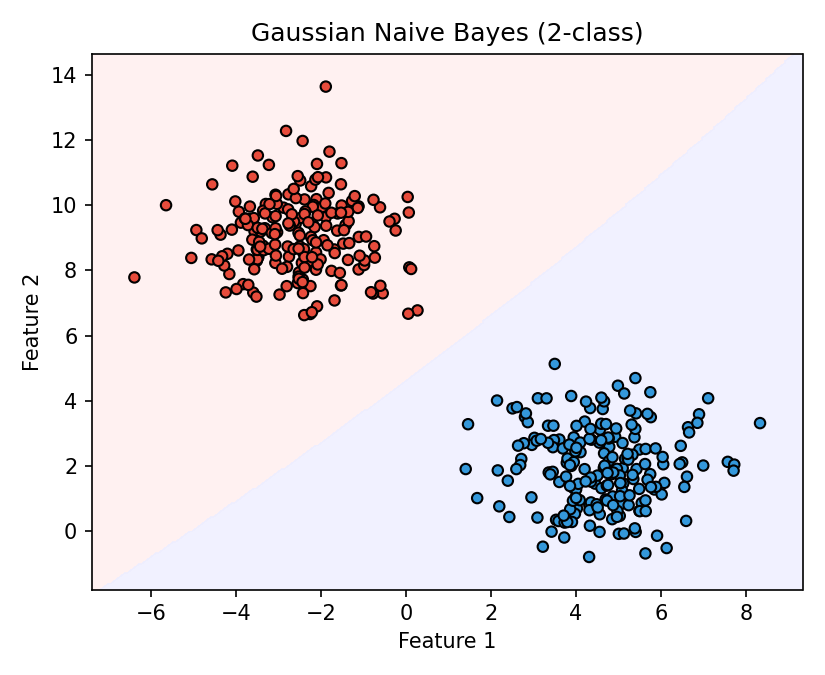
\includegraphics[width=0.9\linewidth]{gnb_decision_boundary_2class.png}
  \caption{Gaussian NB decision boundary (2-class).}
  \label{fig:gnb2}
\end{figure}
\FloatBarrier

\begin{figure}[H]
  \centering
  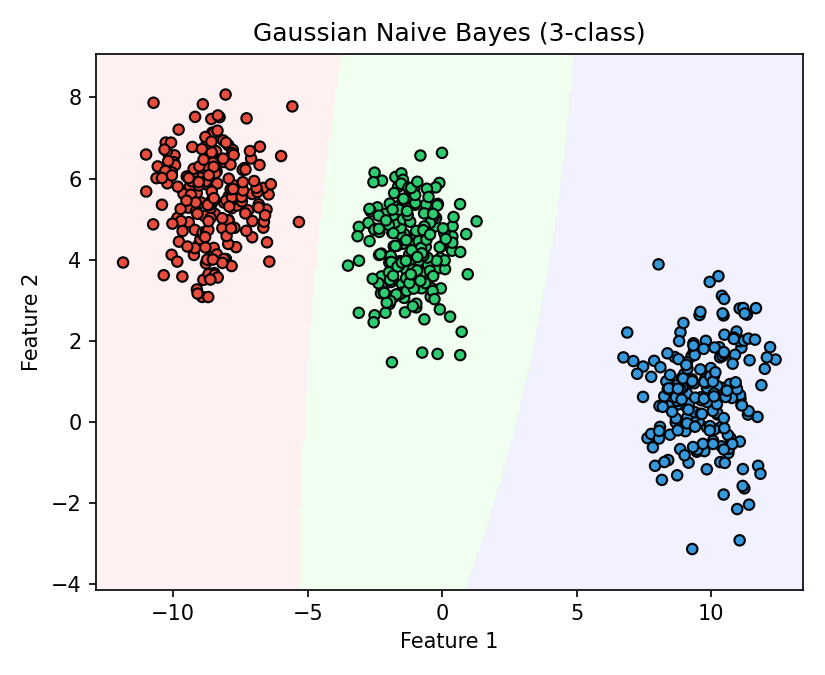
\includegraphics[width=0.9\linewidth]{gnb_decision_boundary_3class.png}
  \caption{Gaussian NB decision regions (3-class).}
  \label{fig:gnb3}
\end{figure}
\FloatBarrier

\begin{figure}[H]
  \centering
  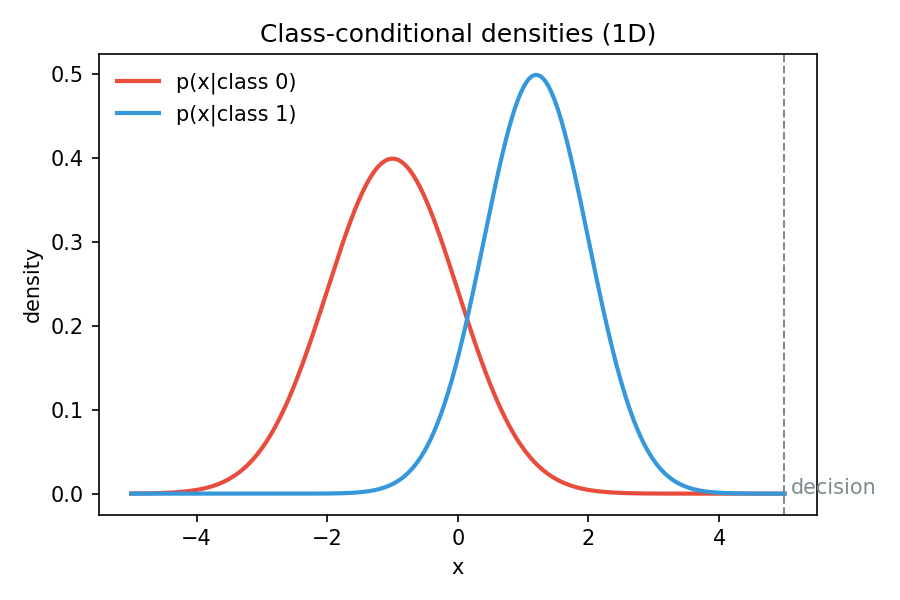
\includegraphics[width=0.9\linewidth]{class_conditional_densities_1d.png}
  \caption{Class-conditional densities in 1D and a decision threshold.}
  \label{fig:dens1d}
\end{figure}
\FloatBarrier

\begin{figure}[H]
  \centering
  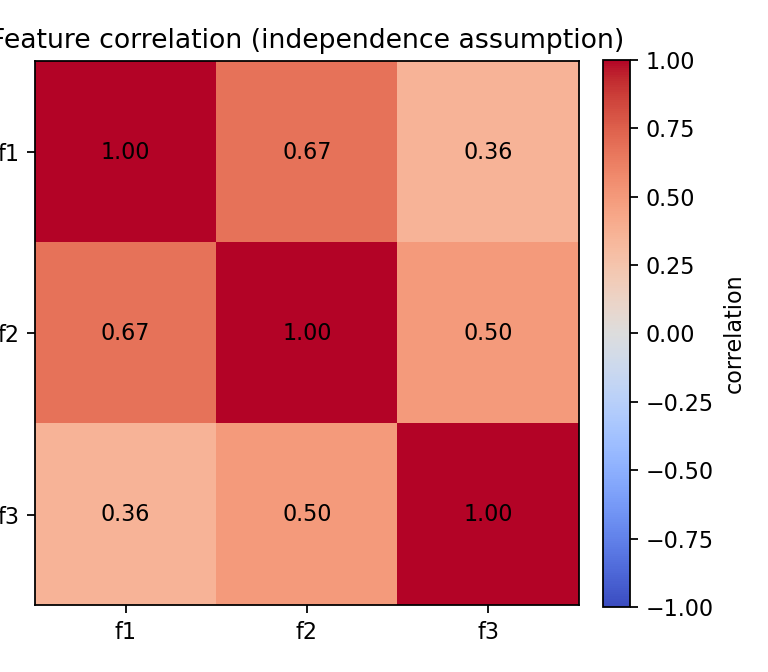
\includegraphics[width=0.9\linewidth]{feature_independence_heatmap.png}
  \caption{Feature correlation heatmap (independence assumption illustration).}
  \label{fig:heatmap}
\end{figure}
\FloatBarrier

\begin{figure}[H]
  \centering
  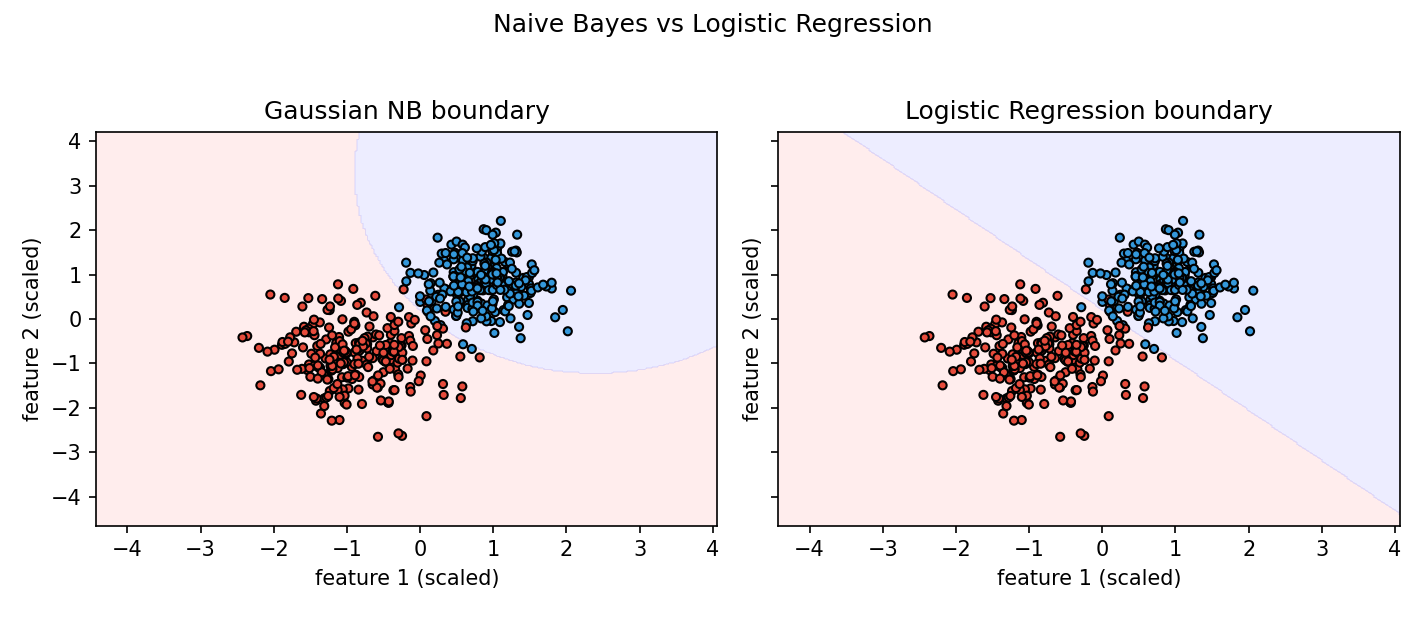
\includegraphics[width=0.95\linewidth]{gnb_vs_logreg_boundary.png}
  \caption{Decision boundary comparison: Gaussian NB vs Logistic Regression.}
  \label{fig:nb_vs_lr}
\end{figure}
\FloatBarrier

\section{Summary}
Na"\i ve Bayes offers a fast, interpretable baseline. Its core idea is simple---combine class priors with per-feature likelihoods under conditional independence. While the assumption is often violated, NB remains competitive on certain problems and serves as a strong baseline against more flexible discriminative models.

\end{document}

